% MC200 revision following the author's November 22 panel sketches.
% Portrait print master: 61 x 85 cm. Figures are generated from stored results.
\documentclass{article}
\usepackage[paperwidth=61cm,paperheight=85cm,margin=0cm]{geometry}
\usepackage[T1]{fontenc}
\usepackage{lmodern}
\usepackage{amsmath,amssymb,graphicx,tikz,xcolor,qrcode,array}
\usepackage[hidelinks]{hyperref}
\renewcommand{\familydefault}{\sfdefault}
\pagestyle{empty}
\definecolor{ink}{HTML}{192F40}
\definecolor{teal}{HTML}{007D80}
\definecolor{pale}{HTML}{EAF4F2}
\definecolor{muted}{HTML}{526674}
\definecolor{line}{HTML}{D8E2E5}
\definecolor{orange}{HTML}{D55E00}
\definecolor{rose}{HTML}{A42B77}
\newcommand{\bodyfont}{\fontsize{18.5}{24}\selectfont}
\newcommand{\captionfont}{\fontsize{17.5}{22}\selectfont}
\newcommand{\detailfont}{\fontsize{16.5}{21}\selectfont}
\newcommand{\sectiontitle}[2]{{\color{teal}\fontsize{19}{23}\selectfont\bfseries #1}\hspace{.18cm}{\color{ink}\fontsize{24}{29}\selectfont\bfseries #2}}
\setlength{\parindent}{0pt}
\setlength{\parskip}{.20cm}
\hypersetup{pdftitle={When does a connectome beat a random reservoir?},pdfauthor={Miles Walter Churchland and collaborators}}
\newdimen\posterheight
\newcommand{\place}[6]{%
  \node[anchor=north west,inner sep=0pt] (#1) at (#2,-#3) {\begin{minipage}[t]{#4cm}\raggedright\color{ink}#6\end{minipage}};%
  \pgfextracty{\posterheight}{\pgfpointdiff{\pgfpointanchor{#1}{south west}}{\pgfpointanchor{#1}{north west}}}%
  \ifdim\posterheight>#5cm
    \PackageWarning{poster}{POSTER LAYOUT: #1 exceeds its #5 cm vertical budget}%
  \fi
  \typeout{POSTER BLOCK #1: height=\the\posterheight, budget=#5cm}%
}
\begin{document}
\null
\begin{tikzpicture}[remember picture,overlay,x=1cm,y=1cm]
\begin{scope}[shift={(current page.north west)}]

% Title and a short motivation line, before the two-pane methods band.
\fill[ink] (0,0) rectangle (61,-10.1);
\fill[teal] (0,-10.1) rectangle (61,-10.3);
\place{event}{2}{.8}{57}{.7}{{\color{white}\fontsize{15}{19}\selectfont\bfseries NEURREPS 2026\hfill CONNECTOME RESERVOIR COMPUTING}}
\place{title}{2}{1.9}{50}{4.8}{{\color{white}\fontsize{67}{74}\selectfont\bfseries When does a connectome\par beat a random reservoir?}}
\place{authors}{2}{6.9}{57}{1.65}{{\color{white}\fontsize{19}{24}\selectfont Miles Walter Churchland\textsuperscript{1}, Raul de Palma Aristides\textsuperscript{2}, Jordi Garcia-Ojalvo\textsuperscript{1},\par Anna Ritz\textsuperscript{3}, Greg Anderson\textsuperscript{4}, Miguel C. Soriano\textsuperscript{2}}}
\place{affiliations}{2}{8.9}{57}{1.0}{{\color{white}\fontsize{13.5}{18}\selectfont \textsuperscript{1}Universitat Pompeu Fabra\quad \textsuperscript{2}IFISC, CSIC--UIB\quad \textsuperscript{3}Biology, Reed College\quad \textsuperscript{4}Computer Science, Reed College}}
\place{code}{54.7}{2.1}{4.3}{4.5}{{\color{white}\fontsize{12}{16}\selectfont\bfseries CODE}\par\vspace{.10cm}\href{https://github.com/mchurchland/Thesis}{\begingroup\setlength{\fboxsep}{2mm}\colorbox{white}{\qrcode[height=2.8cm]{https://github.com/mchurchland/Thesis}}\endgroup}\par\vspace{.10cm}{\color{white}\fontsize{11}{14}\selectfont Models and protocols}}
\place{motivation-title}{2}{11.0}{57}{1.0}{{\color{teal}\fontsize{25}{30}\selectfont\bfseries Does biological wiring help, or do its connection strengths matter more?}}
\place{motivation}{2}{12.35}{57}{1.8}{\bodyfont We compare \textit{C.~elegans} (CE) with random reservoirs across input strength and the fraction of inhibitory edges. Controls separate the placement, topology and distribution of connection strengths.}

% Top band: two panels. These explain the actual protocol, including nested signs.
\draw[line,line width=1pt] (2,-14.2) -- (59,-14.2);
\draw[line,line width=1pt] (30.5,-14.7) -- (30.5,-30.5);
\place{methods-title}{2}{14.8}{27.6}{1.1}{\sectiontitle{}{Methods and sweep}}
\place{methods-intro}{2}{16.2}{27.6}{2.2}{\bodyfont A fixed tanh reservoir receives a scalar input. Only the linear readout is trained: reconstruct past inputs (MC200) or predict a nonlinear sequence (NARMA10).}
\node[draw=line,rounded corners=2pt,fill=pale,text=ink,align=center,font=\fontsize{16}{20}\selectfont,minimum width=5.3cm,minimum height=1.05cm] at (5.3,-19.2) {Input $u(t)$};
\node[draw=line,rounded corners=2pt,fill=pale,text=ink,align=center,font=\fontsize{16}{20}\selectfont,minimum width=8.2cm,minimum height=1.05cm] at (14.7,-19.2) {Fixed recurrent network};
\node[draw=line,rounded corners=2pt,fill=pale,text=ink,align=center,font=\fontsize{16}{20}\selectfont,minimum width=6.0cm,minimum height=1.05cm] at (25.5,-19.2) {Trained readout};
\draw[-latex,muted,line width=1.2pt] (8.1,-19.2) -- (10.2,-19.2);
\draw[-latex,muted,line width=1.2pt] (19.0,-19.2) -- (22.2,-19.2);
\place{sweep-design}{2}{20.65}{14.2}{7.0}{\bodyfont
\textbf{100 paired realizations}\par
\textbf{11 inhibitory fractions:}\par
0--100\%, in 10\% steps\par
\textbf{24 settings:}\par
Radius: $0.6,\ 0.95,\ 1.05$\par
Leak: $0.6,\ 1.0$\par
Input: $0.01,\ 0.1,\ 0.5,\ 1.5$
}
\place{protocol}{16.6}{20.65}{13.0}{7.0}{\bodyfont
\textbf{297 neurons; 3,604 edges} [1]\par
Contact-count magnitudes [1]\par
Chemical edges; bias $=0$\par
Input reaches all nodes\par
Ridge selected on validation\par
Train 1,500 / validation 500\par
Washout 500 time steps\par
Test: MC 5,000 / NARMA 500
}
\place{methods-note}{2}{27.8}{27.6}{2.5}{\captionfont Models share input streams and projections. MC200 sums recall $r^2$ over delays 1--200 [2]. Main results scale each matrix to its own target radius. Bands resample whole paired realizations.}
\place{network-title}{31.3}{14.8}{27.7}{1.1}{\sectiontitle{}{Which edges become inhibitory?}}
\place{network}{31.3}{16.1}{27.7}{11.0}{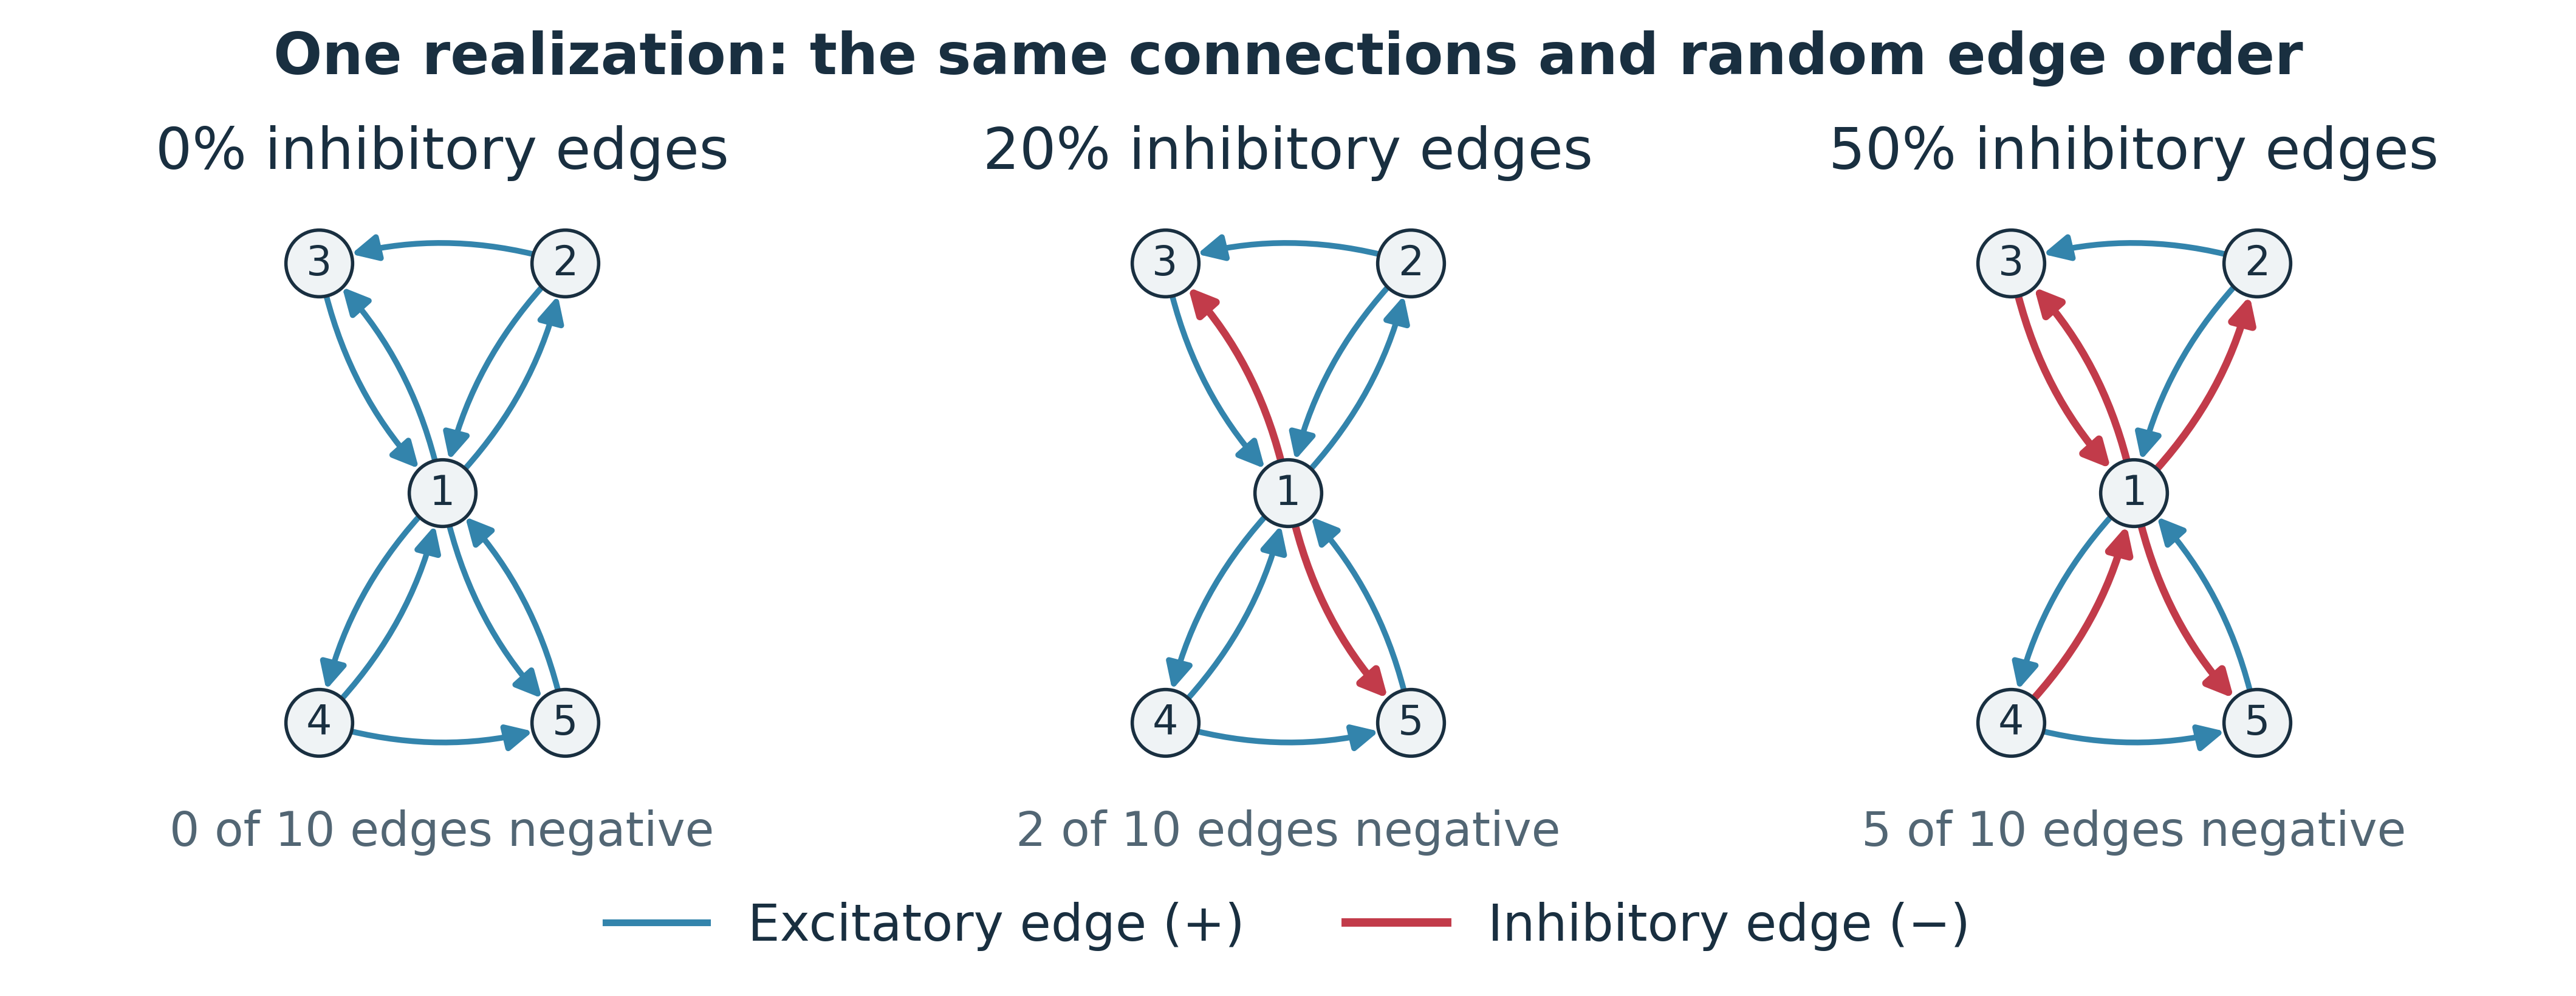
\includegraphics[width=27.7cm]{assets/poster_edge_sign_sweep.png}}
\place{network-caption}{31.3}{27.35}{27.7}{3.1}{\captionfont \textbf{The fraction counts edges, not inhibitory neurons.} Increasing the fraction adds inhibitory edges along one random order; earlier inhibitory edges stay inhibitory. The order is redrawn for each of the 100 realizations.\par
\textit{Five-node, ten-edge illustration; not a CE subgraph.}}

% Middle row: MC only. Three panels follow the author's sketch.
\draw[line,line width=1pt] (2,-31.3) -- (59,-31.3);
\draw[line,line width=1pt] (20.8,-32.0) -- (20.8,-81.4);
\draw[line,line width=1pt] (40.2,-32.0) -- (40.2,-81.4);
\place{mc-title}{2}{32.1}{18.2}{1.1}{\sectiontitle{1.}{Input drive and inhibition}}
\place{mc-subtitle}{2}{33.45}{18.2}{1.2}{\captionfont Own-radius scaling; inputs 0.01 and 0.5}
\place{mc-curves}{2}{34.6}{18.2}{16.6}{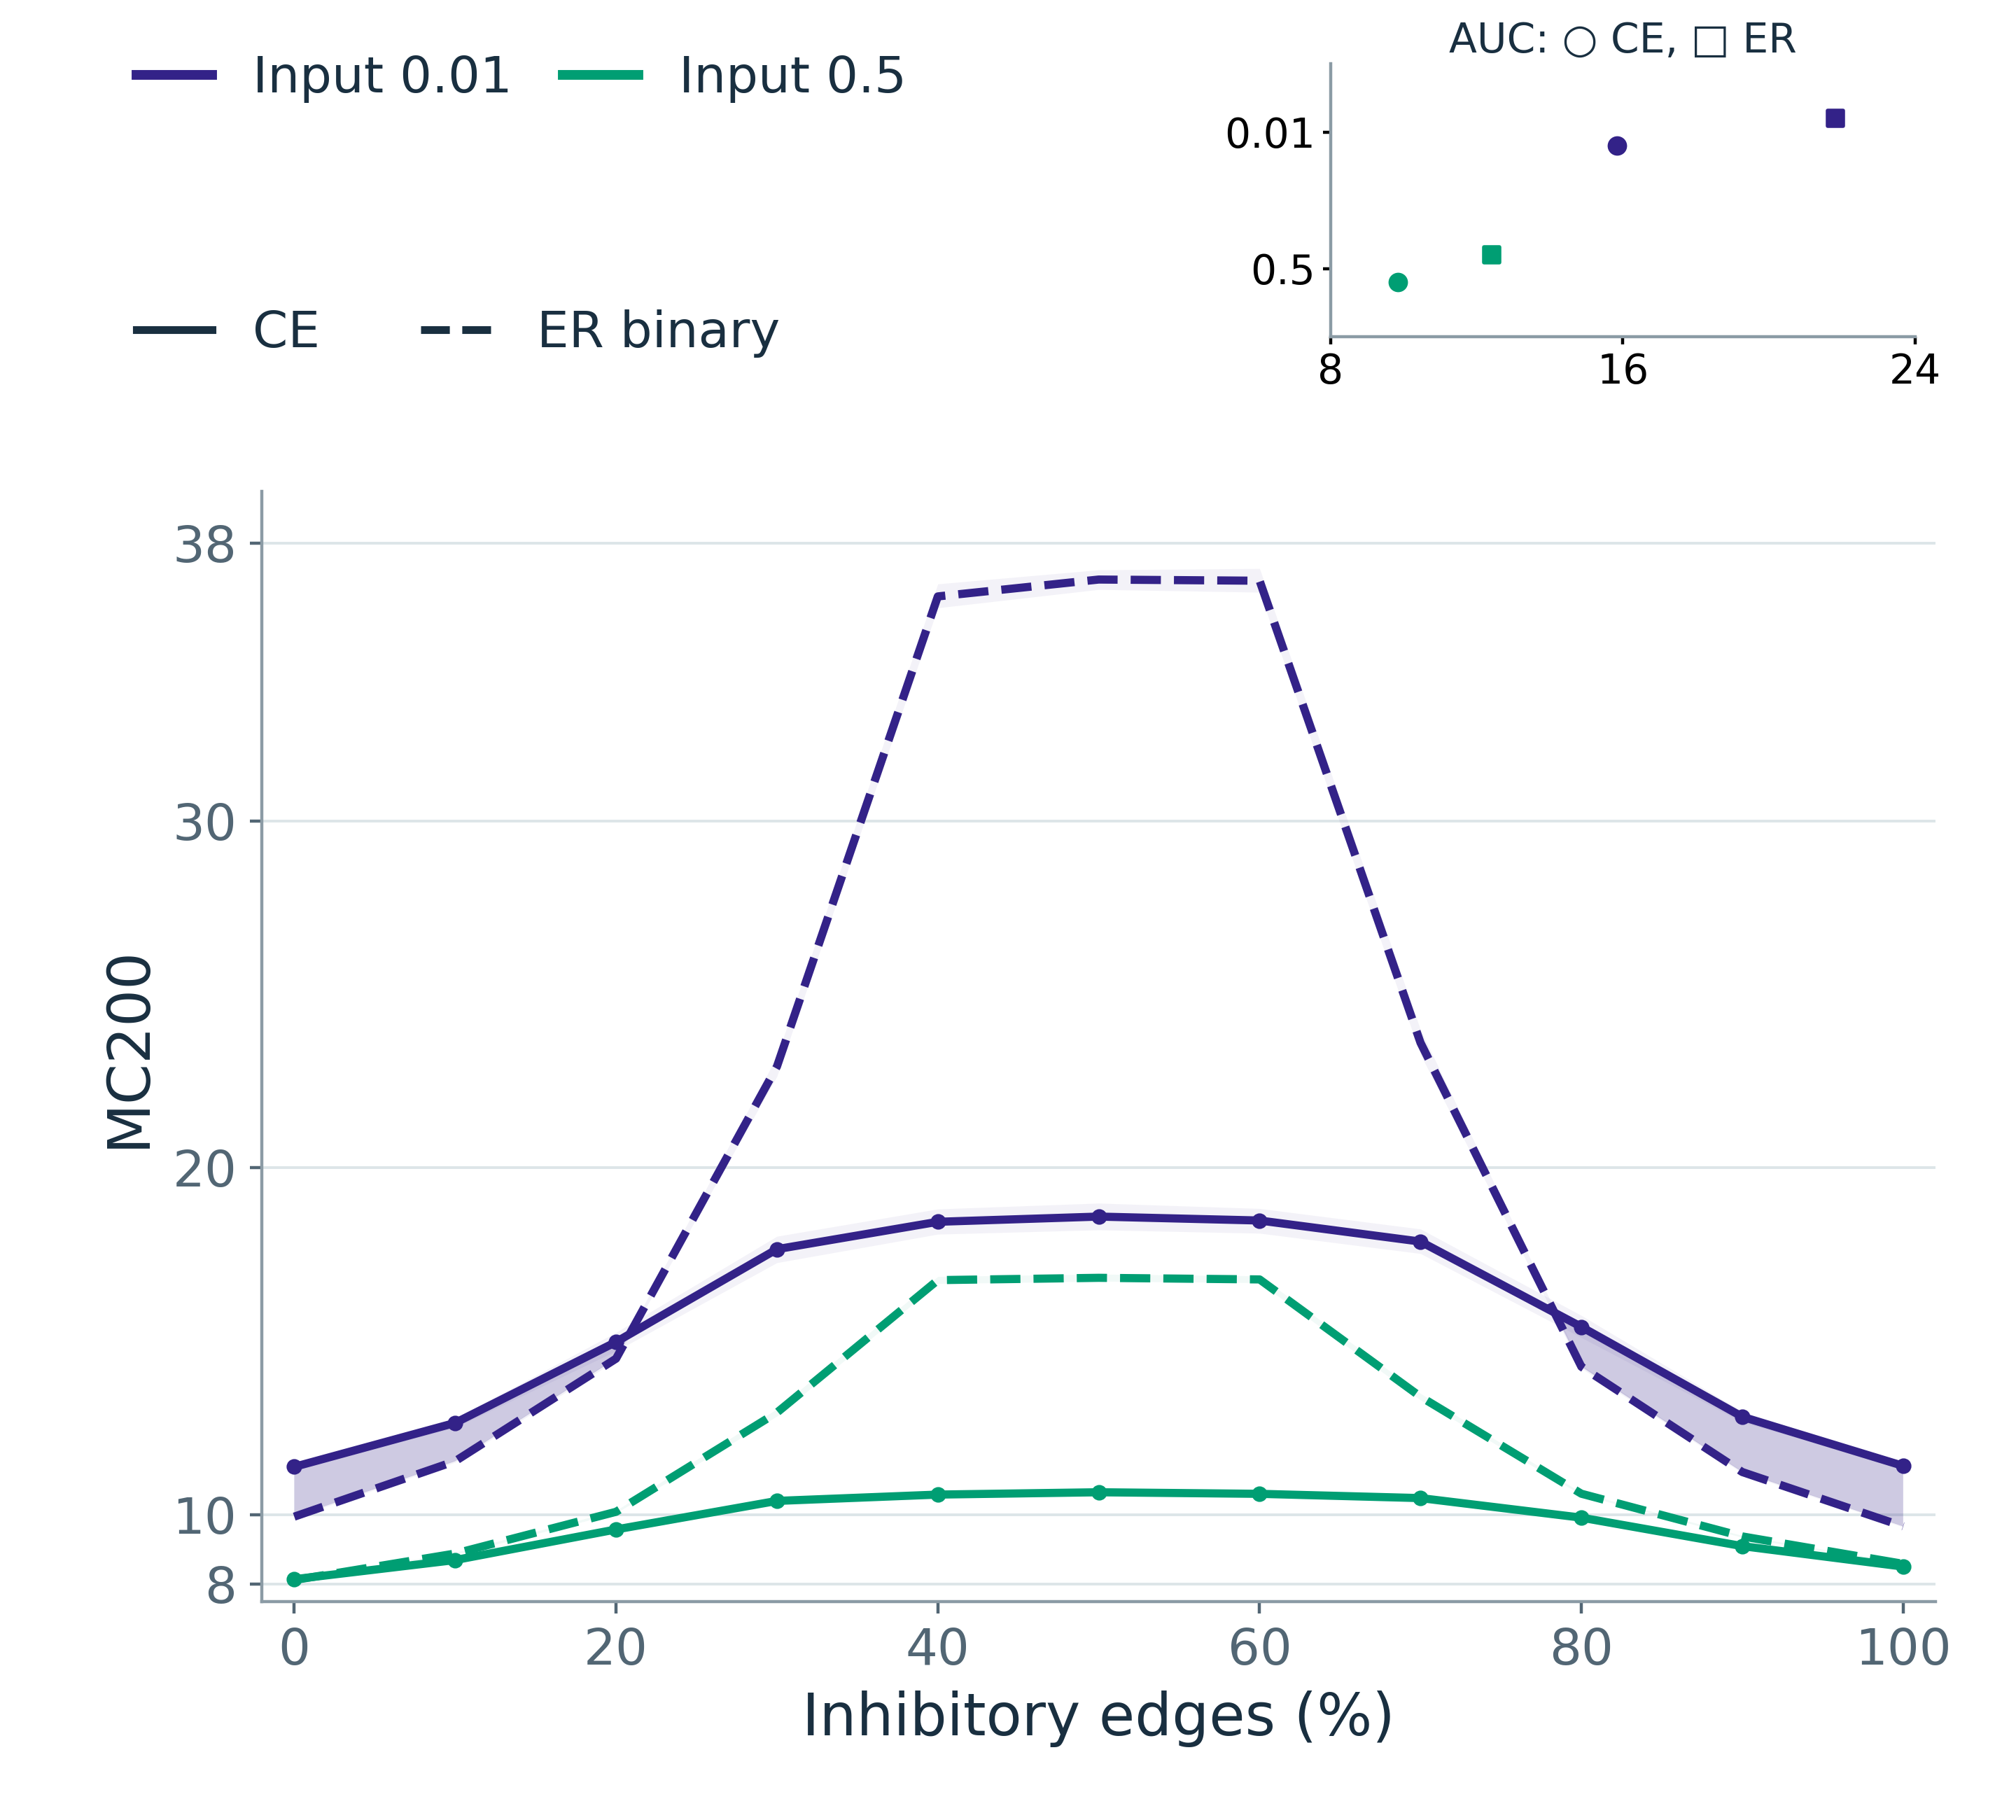
\includegraphics[width=18.2cm]{assets/poster_mc_input_curves.png}}
\place{mc-caption}{2}{51.6}{18.2}{3.3}{\bodyfont CE's advantage over binary ER is strongest under weak input at the extremes. Fill marks where CE leads; the inset shows AUC for each input. Each curve averages six radius/leak settings.}
\fill[pale] (2,-55.2) rectangle (20.2,-57.45);
\place{mc-callout}{2.4}{55.5}{17.4}{1.8}{\captionfont Across all 24 settings, mean MC AUC is \textbf{11.39 for CE} versus \textbf{14.93 for binary ER}.}

\place{structure-title}{21.4}{32.1}{18.2}{1.1}{\sectiontitle{2.}{Placement and topology}}
\place{structure-subtitle}{21.4}{33.45}{18.2}{1.2}{\captionfont Mean MC200 AUC; own-radius scaling}
\place{structure-figure}{21.4}{34.8}{18.2}{15.4}{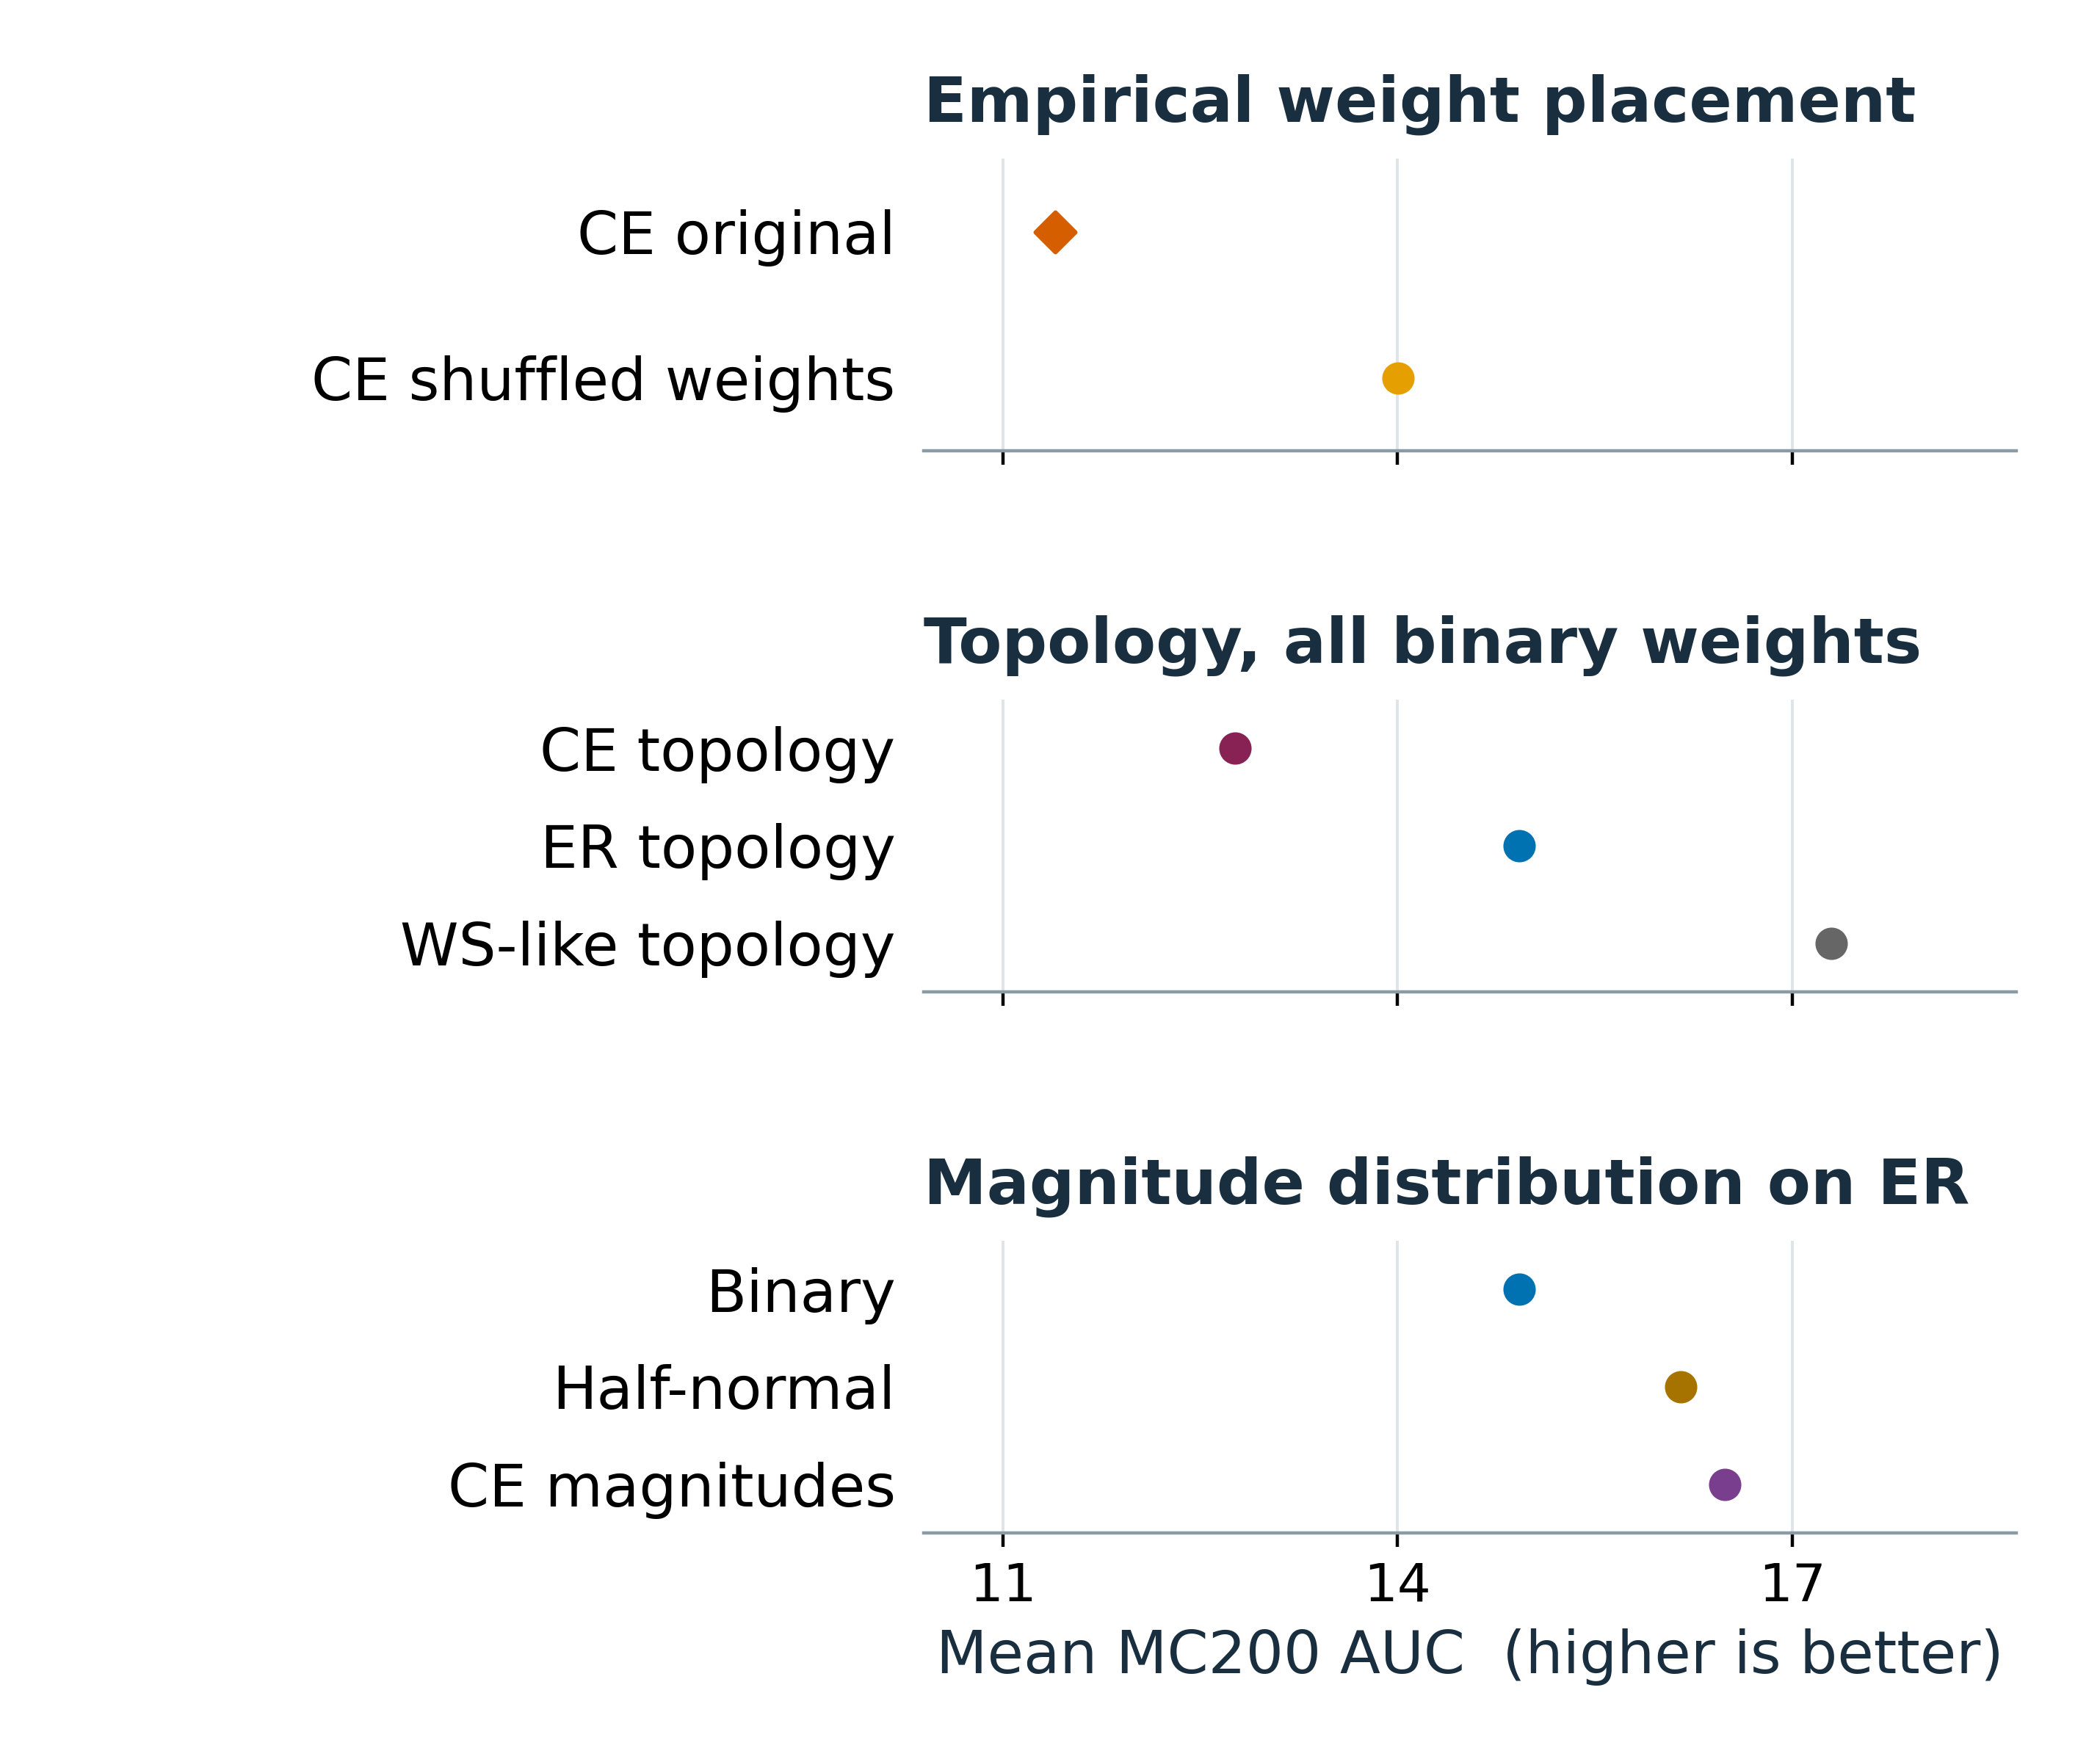
\includegraphics[width=18.2cm]{assets/poster_structural_mc_auc.png}}
\place{structure-caption}{21.4}{50.7}{18.2}{6.6}{\bodyfont
\textbf{Placement:} reassigning CE's weights improves mean MC.\par
\textbf{Topology:} under own-radius scaling, binary CE performs below binary ER and WS-like networks.\par
\textbf{Distribution:} on ER, CE magnitudes outperform binary and half-normal weights in aggregate.
}

\place{weights-title}{40.8}{32.1}{18.2}{1.1}{\sectiontitle{3.}{Which weight features help?}}
\place{weight-pipeline}{40.8}{33.65}{18.2}{1.3}{{\color{muted}\fontsize{16.5}{21}\selectfont Same ER edges, signs and inputs.\par Change the magnitude distribution.}}
\place{weights-figure}{40.8}{35.6}{18.2}{14.3}{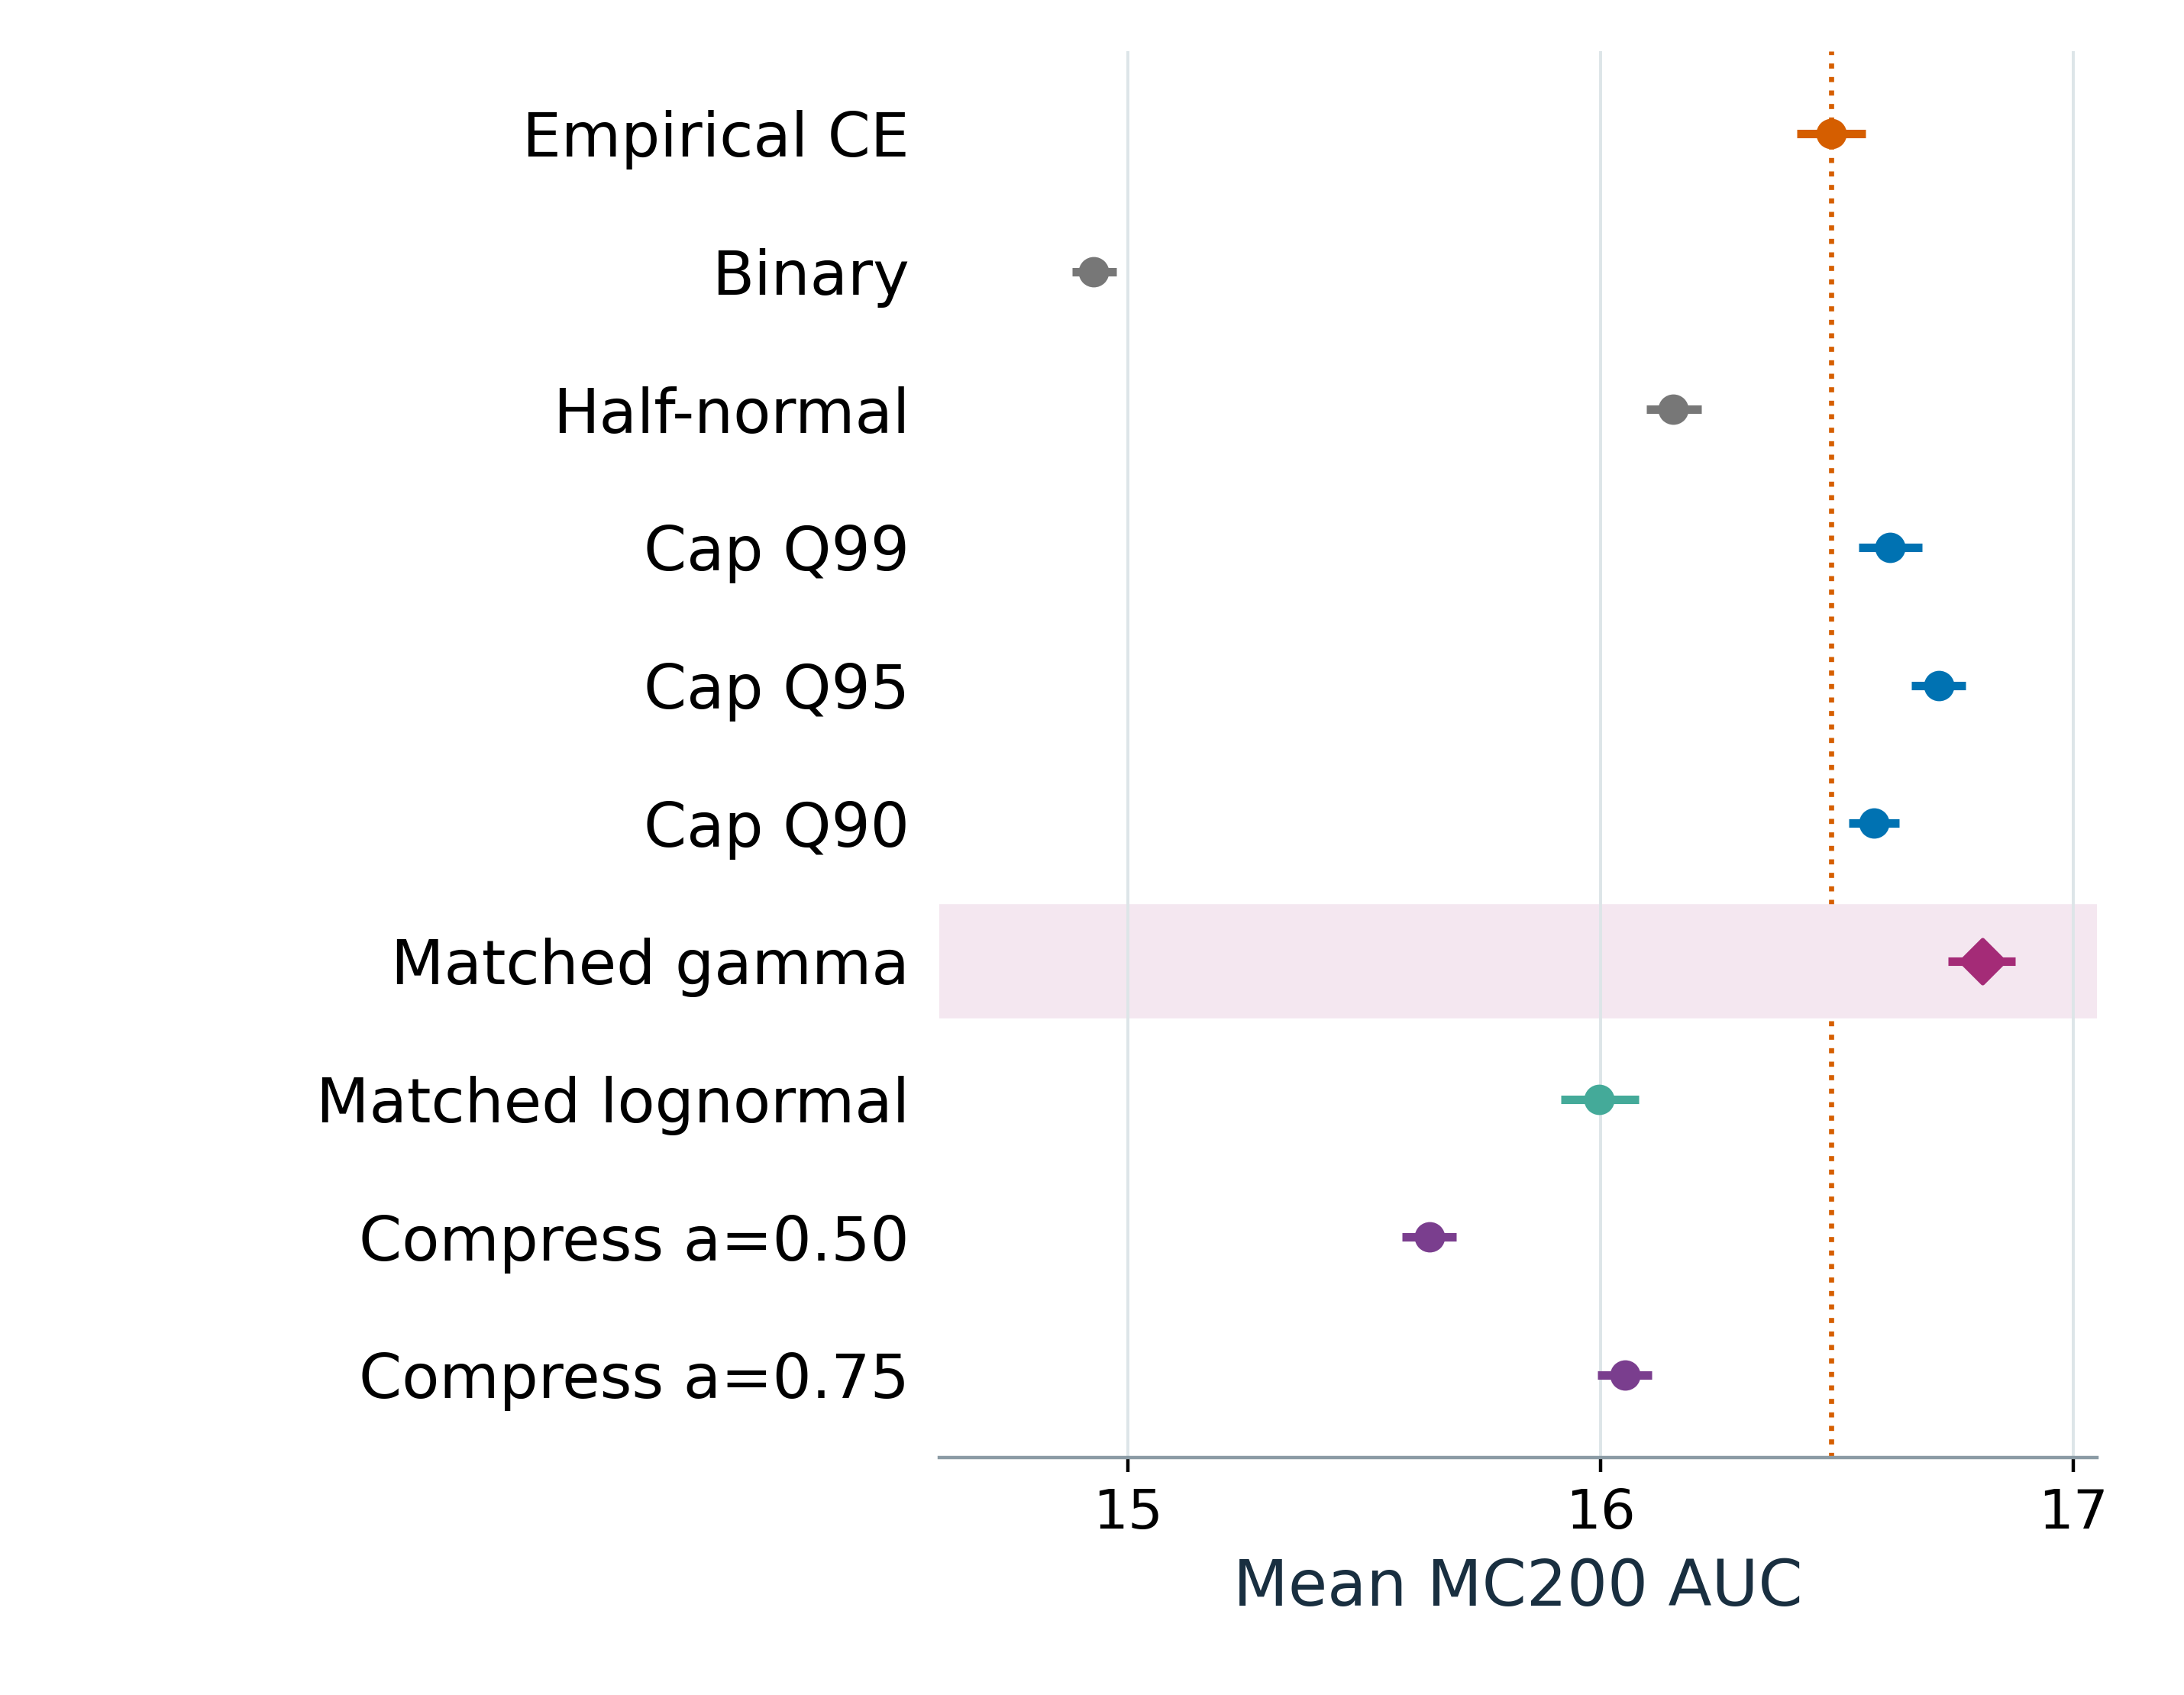
\includegraphics[width=18.2cm]{assets/poster_er_weight_mc_auc.png}}
\place{weights-caption}{40.8}{50.4}{18.2}{4.2}{\bodyfont \textbf{Gamma improves mean MC by 1.94\%:}\par
$+0.320$ [95\% CI: $0.296,\ 0.345$].\par
Upper-tail caps also improve MC200. Compressing the spread or matching a lognormal worsens it.}
\place{weights-note}{40.8}{55.0}{18.2}{2.4}{\captionfont Gamma and lognormal match CE's mean and variance. \textbf{Those two moments alone do not explain performance.} Caps restore mean magnitude.}

% Bottom row: NARMA replication, critics' corner, then conclusions.
\draw[line,line width=1pt] (2,-58.35) -- (59,-58.35);
\place{narma-title}{2}{59.2}{18.2}{1.1}{\sectiontitle{4.}{The result extends to NARMA}}
\place{narma-subtitle}{2}{60.65}{18.2}{.9}{\captionfont Prediction error; own-radius scaling}
\place{narma-figure}{2}{61.7}{18.2}{17.9}{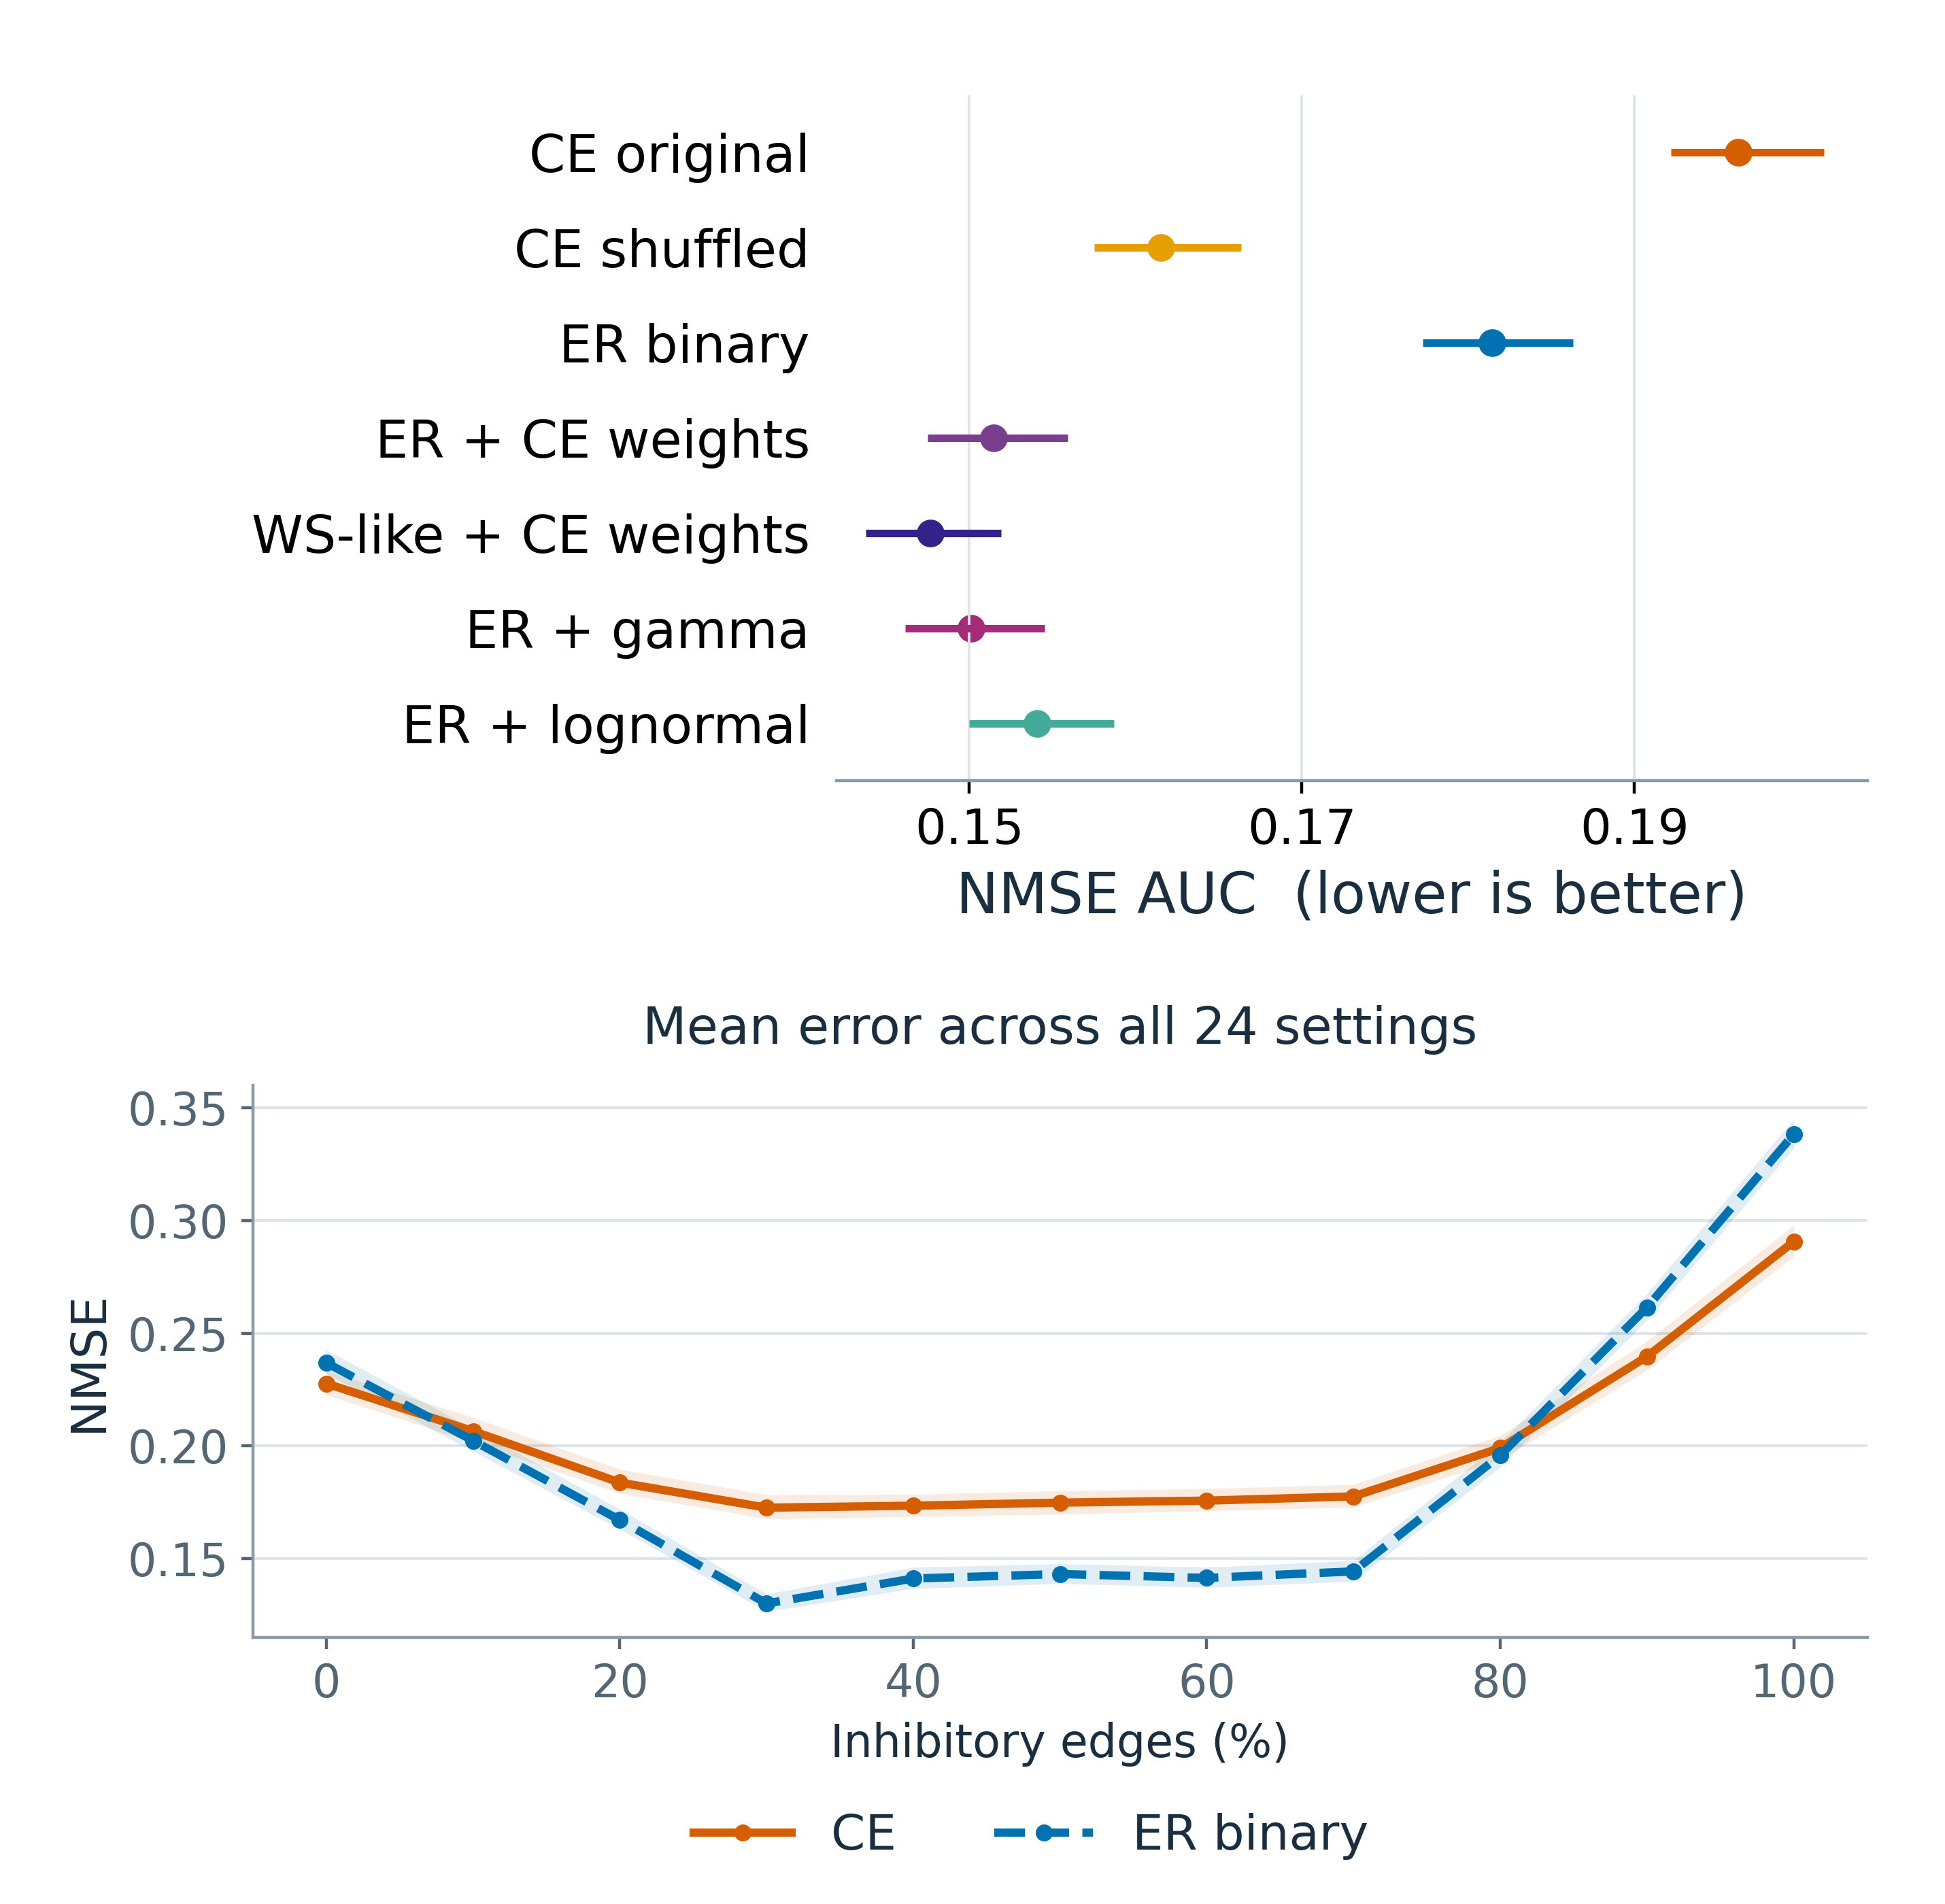
\includegraphics[width=18.2cm]{assets/poster_narma.png}}
\place{narma-caption}{2}{79.9}{18.2}{1.7}{\captionfont Reassigning weights helps; gamma reduces ER's error AUC by \textbf{0.89\%}. NARMA uses the archived paired runs.}

\place{critics-title}{21.4}{59.2}{18.2}{1.1}{\sectiontitle{5.}{Critics' corner}}
\place{critics-scaling}{21.4}{60.75}{18.2}{3.2}{\bodyfont Normalizing to the same radius changes each matrix's effective weights:\par
\hfill$\widehat W=\rho_{\rm target} W/\rho(W)$.\hfill\null\par
A shared multiplier reverses the average CE-versus-ER binary ranking.}
\place{critics-figure}{21.4}{64.4}{18.2}{8.6}{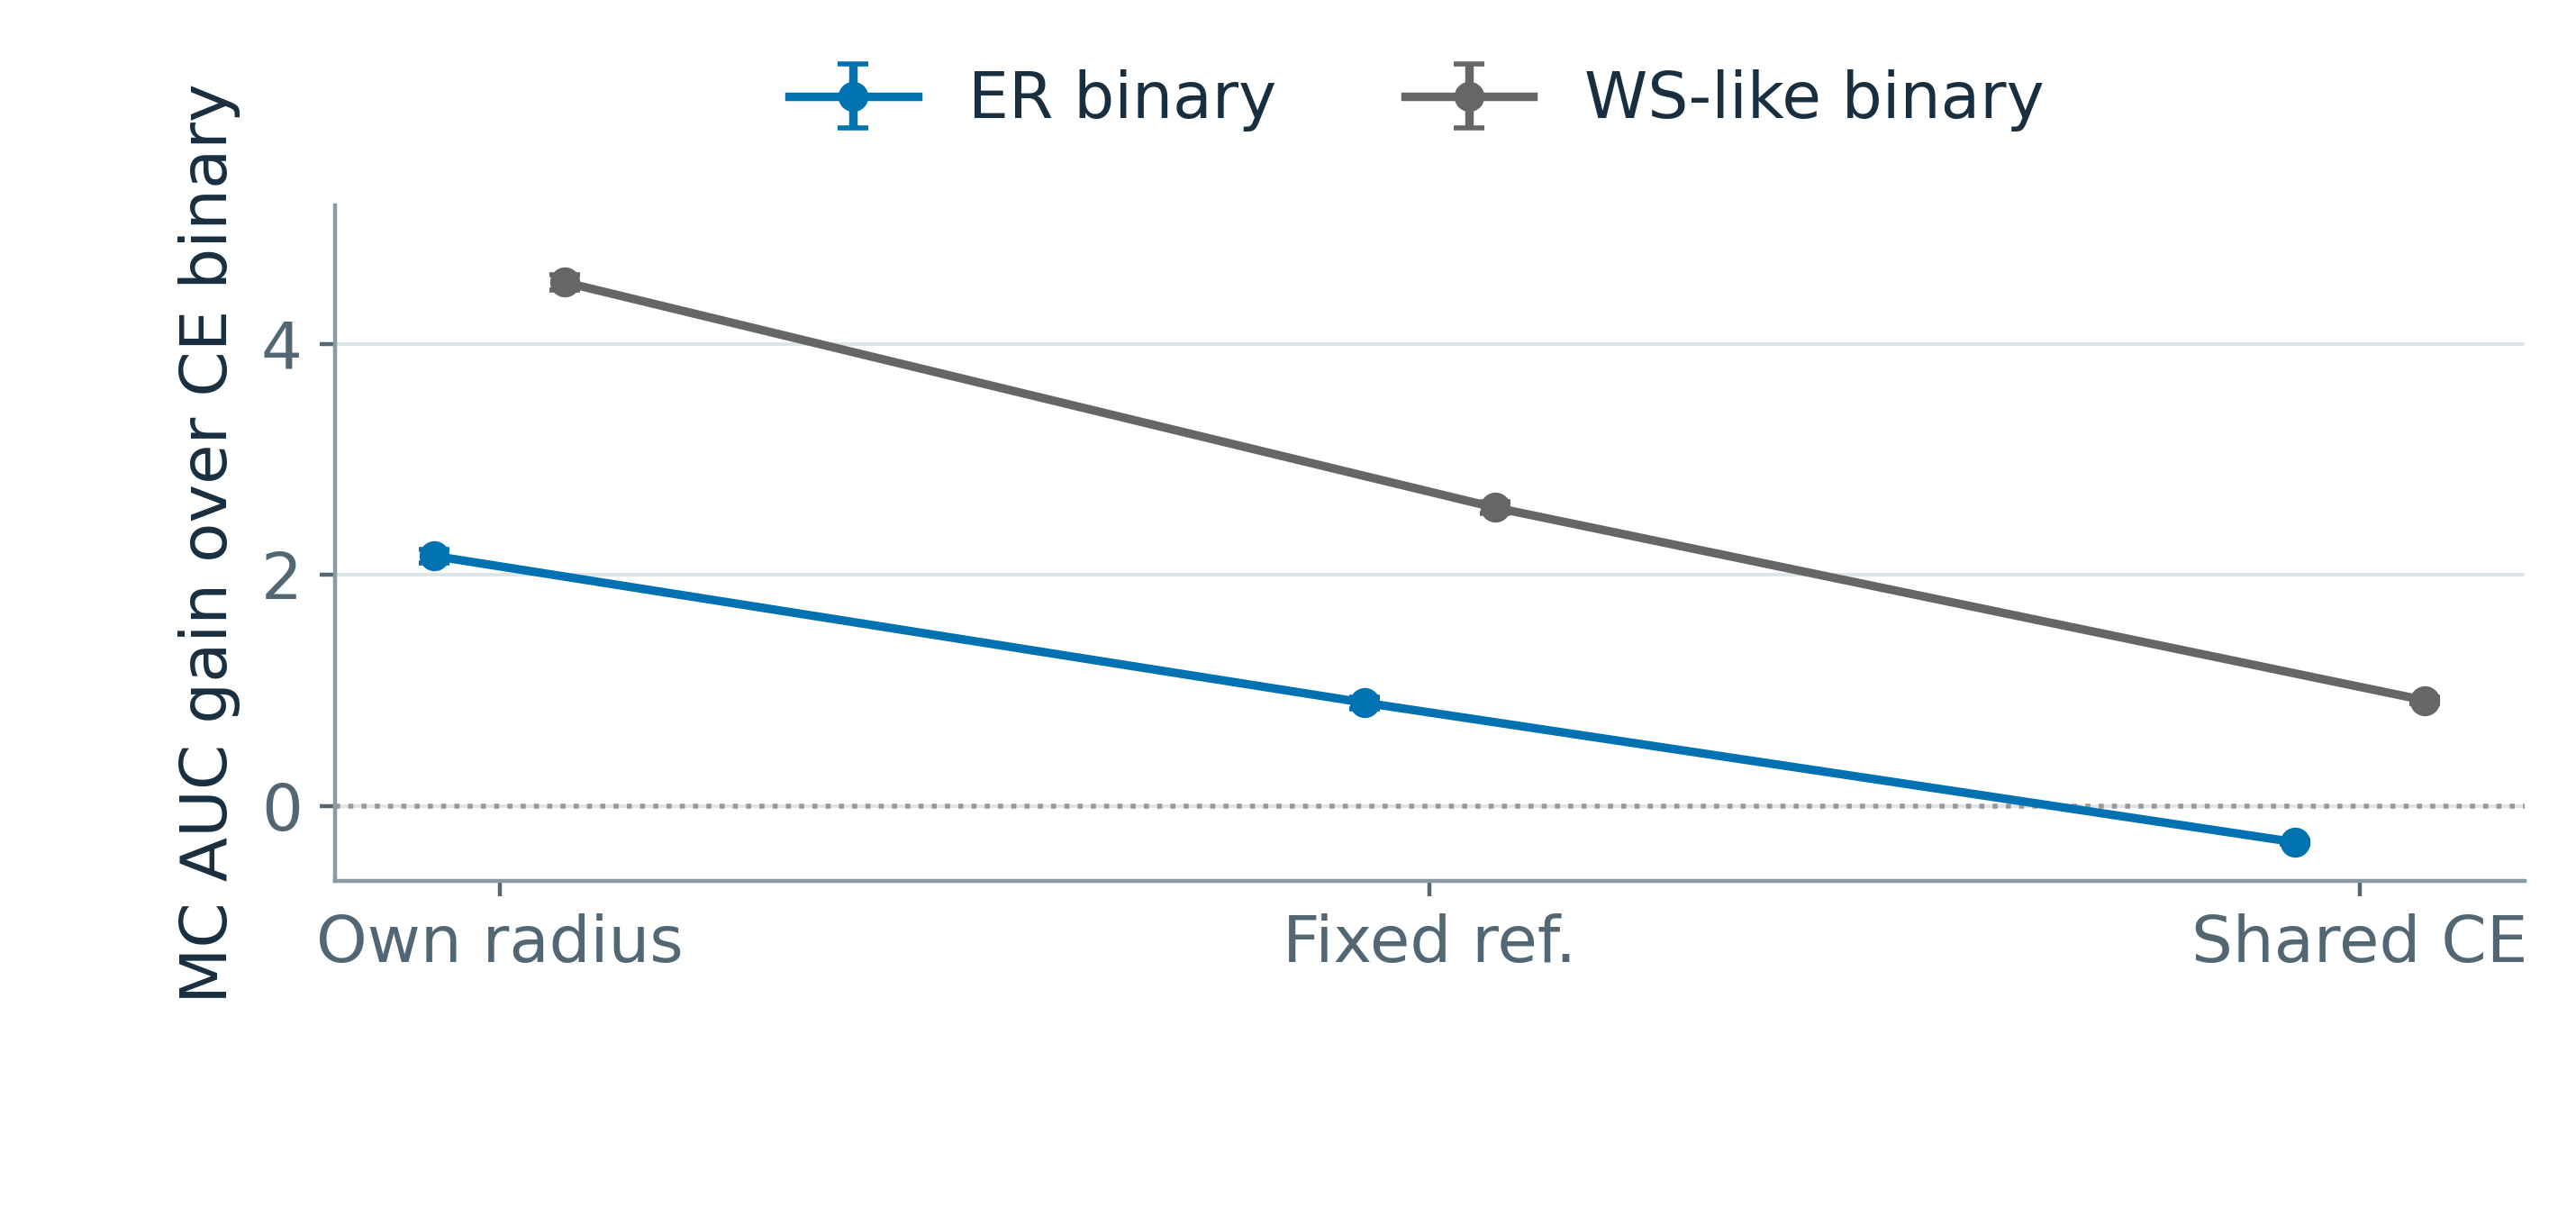
\includegraphics[width=18.2cm]{assets/poster_normalization_caveat.png}}
\place{peak-title}{21.4}{73.3}{18.2}{1.0}{{\fontsize{21}{26}\selectfont\bfseries Mean AUC $\ne$ peak performance}}
\place{peak-intro}{21.4}{74.55}{18.2}{1.0}{\captionfont Top three models and CE; own-radius scaling:}
\place{peak-order}{21.4}{75.7}{18.2}{4.3}{{\fontsize{18}{22}\selectfont\setlength{\tabcolsep}{3pt}\renewcommand{\arraystretch}{1.04}
\begin{tabular}{@{}p{10.7cm}r@{}}
\textbf{Model (rank)} & \textbf{Peak MC200}\\
1. WS binary & 70.88\\
2. ER binary & 67.62\\
3. WS half-normal & 67.19\\
11. CE original & 24.13
\end{tabular}}}
\place{peak-note}{21.4}{80.0}{18.2}{1.4}{\detailfont Maxima of seed-mean test scores: descriptive grid peaks, not independently validated tuning.}

\place{conclusions-title}{40.8}{59.2}{18.2}{1.1}{\sectiontitle{6.}{Conclusions}}
\place{conclusions-lead}{40.8}{60.85}{18.2}{2.5}{{\color{teal}\fontsize{25}{31}\selectfont\bfseries Biological wiring is not a general advantage here.}}
\place{conclusions}{40.8}{64.1}{18.2}{10.4}{\bodyfont
\textbf{1.} CE wins limited conditions against binary ER. Stronger weight-matched controls remove its MC advantage under own-radius scaling.\par\vspace{.35cm}
\textbf{2.} Under own-radius scaling, CE weight placement and topology limit mean performance. Its magnitude distribution remains useful when transferred to \textbf{both ER and WS-like networks}.\par\vspace{.35cm}
\textbf{3.} A matched gamma improves ER memory and prediction. The distributional features driving this gain remain to be isolated.
}
\fill[pale] (40.8,-75.6) rectangle (59,-78.65);
\place{conclusions-takehome}{41.25}{76.0}{17.3}{2.3}{{\fontsize{21}{27}\selectfont\bfseries Identify which features of a biological substrate provide a computational advantage.}}
\place{conclusions-scope}{40.8}{79.2}{18.2}{2.3}{\captionfont These are conditional reservoir results, not claims about the worm's natural memory or biological E/I balance.}

\draw[line,line width=1pt] (2,-82.1) -- (59,-82.1);
\place{references}{2}{82.55}{57}{2.0}{{\color{muted}\fontsize{12.5}{16}\selectfont
[1] Fenyves et al. (2020), \textit{PLOS Comput. Biol.} 16:e1007974.\quad
[2] Jaeger (2002), \textit{Short Term Memory in Echo State Networks}.\par
AUC: trapezoidal E/I integral divided by sweep width; equal weight per grid setting. Intervals: 1,000 whole-realization bootstrap draws; exploratory.\par
Static tanh reservoirs; randomized chemical-edge signs; no electrical synapses. WS denotes the directed WS-like control. Compute: Orca, Portland State University.}}
\end{scope}
\end{tikzpicture}
\end{document}
